%\documentclass[slides]{beamer} %switch "slides" to "handout" for printing out
\documentclass[handout]{beamer}

%packages
%\usepackage{latexsym}
\usepackage{graphicx}
\usepackage{color}
\usepackage{amsmath}
\usepackage{dsfont}
\usepackage{placeins}
\usepackage{amssymb}
\usepackage{wasysym}
\usepackage{abstract}
\usepackage{hyperref}
\usepackage{etoolbox}
\usepackage{datetime}
\usepackage{xcolor}
\usepackage{alphalph}
\settimeformat{ampmtime}

%\usepackage{pstricks,pst-node,pst-tree}

%\usepackage{algpseudocode}
%\usepackage{amsthm}
%\usepackage{hyperref}
%\usepackage{mathrsfs}
%\usepackage{amsfonts}
%\usepackage{bbding}
%\usepackage{listings}
%\usepackage{appendix}
\usepackage[margin=1in]{geometry}
%\geometry{papersize={8.5in,11in},total={6.5in,9in}}
%\usepackage{cancel}
%\usepackage{algorithmic, algorithm}

\makeatletter
\def\maxwidth{ %
  \ifdim\Gin@nat@width>\linewidth
    \linewidth
  \else
    \Gin@nat@width
  \fi
}
\makeatother

\definecolor{fgcolor}{rgb}{0.345, 0.345, 0.345}
\newcommand{\hlnum}[1]{\textcolor[rgb]{0.686,0.059,0.569}{#1}}%
\newcommand{\hlstr}[1]{\textcolor[rgb]{0.192,0.494,0.8}{#1}}%
\newcommand{\hlcom}[1]{\textcolor[rgb]{0.678,0.584,0.686}{\textit{#1}}}%
\newcommand{\hlopt}[1]{\textcolor[rgb]{0,0,0}{#1}}%
\newcommand{\hlstd}[1]{\textcolor[rgb]{0.345,0.345,0.345}{#1}}%
\newcommand{\hlkwa}[1]{\textcolor[rgb]{0.161,0.373,0.58}{\textbf{#1}}}%
\newcommand{\hlkwb}[1]{\textcolor[rgb]{0.69,0.353,0.396}{#1}}%
\newcommand{\hlkwc}[1]{\textcolor[rgb]{0.333,0.667,0.333}{#1}}%
\newcommand{\hlkwd}[1]{\textcolor[rgb]{0.737,0.353,0.396}{\textbf{#1}}}%

\usepackage{framed}
\makeatletter
\newenvironment{kframe}{%
 \def\at@end@of@kframe{}%
 \ifinner\ifhmode%
  \def\at@end@of@kframe{\end{minipage}}%
  \begin{minipage}{\columnwidth}%
 \fi\fi%
 \def\FrameCommand##1{\hskip\@totalleftmargin \hskip-\fboxsep
 \colorbox{shadecolor}{##1}\hskip-\fboxsep
     % There is no \\@totalrightmargin, so:
     \hskip-\linewidth \hskip-\@totalleftmargin \hskip\columnwidth}%
 \MakeFramed {\advance\hsize-\width
   \@totalleftmargin\z@ \linewidth\hsize
   \@setminipage}}%
 {\par\unskip\endMakeFramed%
 \at@end@of@kframe}
\makeatother

\definecolor{shadecolor}{rgb}{.77, .77, .77}
\definecolor{messagecolor}{rgb}{0, 0, 0}
\definecolor{warningcolor}{rgb}{1, 0, 1}
\definecolor{errorcolor}{rgb}{1, 0, 0}
\newenvironment{knitrout}{}{} % an empty environment to be redefined in TeX

\usepackage{alltt}
\usepackage[T1]{fontenc}

\newcommand{\qu}[1]{``#1''}
\newcounter{probnum}
\setcounter{probnum}{1}

%create definition to allow local margin changes
\def\changemargin#1#2{\list{}{\rightmargin#2\leftmargin#1}\item[]}
\let\endchangemargin=\endlist 

%allow equations to span multiple pages
\allowdisplaybreaks

%define colors and color typesetting conveniences
\definecolor{gray}{rgb}{0.5,0.5,0.5}
\definecolor{black}{rgb}{0,0,0}
\definecolor{white}{rgb}{1,1,1}
\definecolor{blue}{rgb}{0.5,0.5,1}
\newcommand{\inblue}[1]{\color{blue}#1 \color{black}}
\definecolor{green}{rgb}{0.133,0.545,0.133}
\newcommand{\ingreen}[1]{\color{green}#1 \color{black}}
\definecolor{yellow}{rgb}{1,1,0}
\newcommand{\inyellow}[1]{\color{yellow}#1 \color{black}}
\definecolor{orange}{rgb}{0.9,0.649,0}
\newcommand{\inorange}[1]{\color{orange}#1 \color{black}}
\definecolor{red}{rgb}{1,0.133,0.133}
\newcommand{\inred}[1]{\color{red}#1 \color{black}}
\definecolor{purple}{rgb}{0.58,0,0.827}
\newcommand{\inpurple}[1]{\color{purple}#1 \color{black}}
\definecolor{backgcode}{rgb}{0.97,0.97,0.8}
\definecolor{Brown}{cmyk}{0,0.81,1,0.60}
\definecolor{OliveGreen}{cmyk}{0.64,0,0.95,0.40}
\definecolor{CadetBlue}{cmyk}{0.62,0.57,0.23,0}

%define new math operators
\DeclareMathOperator*{\argmax}{arg\,max~}
\DeclareMathOperator*{\argmin}{arg\,min~}
\DeclareMathOperator*{\argsup}{arg\,sup~}
\DeclareMathOperator*{\arginf}{arg\,inf~}
\DeclareMathOperator*{\convolution}{\text{\Huge{$\ast$}}}
\newcommand{\infconv}[2]{\convolution^\infty_{#1 = 1} #2}
%true functions

%%%% GENERAL SHORTCUTS

%shortcuts for pure typesetting conveniences
\newcommand{\bv}[1]{\boldsymbol{#1}}

%shortcuts for compound constants
\newcommand{\BetaDistrConst}{\dfrac{\Gamma(\alpha + \beta)}{\Gamma(\alpha)\Gamma(\beta)}}
\newcommand{\NormDistrConst}{\dfrac{1}{\sqrt{2\pi\sigma^2}}}

%shortcuts for conventional symbols
\newcommand{\tsq}{\tau^2}
\newcommand{\tsqh}{\hat{\tau}^2}
\newcommand{\sigsq}{\sigma^2}
\newcommand{\sigsqsq}{\parens{\sigma^2}^2}
\newcommand{\sigsqovern}{\dfrac{\sigsq}{n}}
\newcommand{\tausq}{\tau^2}
\newcommand{\tausqalpha}{\tau^2_\alpha}
\newcommand{\tausqbeta}{\tau^2_\beta}
\newcommand{\tausqsigma}{\tau^2_\sigma}
\newcommand{\betasq}{\beta^2}
\newcommand{\sigsqvec}{\bv{\sigma}^2}
\newcommand{\sigsqhat}{\hat{\sigma}^2}
\newcommand{\sigsqhatmlebayes}{\sigsqhat_{\text{Bayes, MLE}}}
\newcommand{\sigsqhatmle}[1]{\sigsqhat_{#1, \text{MLE}}}
\newcommand{\bSigma}{\bv{\Sigma}}
\newcommand{\bSigmainv}{\bSigma^{-1}}
\newcommand{\thetavec}{\bv{\theta}}
\newcommand{\thetahat}{\hat{\theta}}
\newcommand{\thetahatmle}{\hat{\theta}_{\mathrm{MLE}}}
\newcommand{\thetavechatmle}{\hat{\thetavec}_{\mathrm{MLE}}}
\newcommand{\muhat}{\hat{\mu}}
\newcommand{\musq}{\mu^2}
\newcommand{\muvec}{\bv{\mu}}
\newcommand{\muhatmle}{\muhat_{\text{MLE}}}
\newcommand{\lambdahat}{\hat{\lambda}}
\newcommand{\lambdahatmle}{\lambdahat_{\text{MLE}}}
\newcommand{\etavec}{\bv{\eta}}
\newcommand{\alphavec}{\bv{\alpha}}
\newcommand{\minimaxdec}{\delta^*_{\mathrm{mm}}}
\newcommand{\ybar}{\bar{y}}
\newcommand{\xbar}{\bar{x}}
\newcommand{\Xbar}{\bar{X}}
\newcommand{\phat}{\hat{p}}
\newcommand{\Phat}{\hat{P}}
\newcommand{\Zbar}{\bar{Z}}
\newcommand{\iid}{~{\buildrel iid \over \sim}~}
\newcommand{\inddist}{~{\buildrel ind \over \sim}~}
\newcommand{\approxdist}{~{\buildrel approx \over \sim}~}
\newcommand{\equalsindist}{~{\buildrel d \over =}~}
\newcommand{\loglik}[1]{\ell\parens{#1}}
\newcommand{\thetahatkminone}{\thetahat^{(k-1)}}
\newcommand{\thetahatkplusone}{\thetahat^{(k+1)}}
\newcommand{\thetahatk}{\thetahat^{(k)}}
\newcommand{\half}{\frac{1}{2}}
\newcommand{\third}{\frac{1}{3}}
\newcommand{\twothirds}{\frac{2}{3}}
\newcommand{\fourth}{\frac{1}{4}}
\newcommand{\fifth}{\frac{1}{5}}
\newcommand{\sixth}{\frac{1}{6}}

%shortcuts for vector and matrix notation
\newcommand{\A}{\bv{A}}
\newcommand{\At}{\A^T}
\newcommand{\Ainv}{\inverse{\A}}
\newcommand{\B}{\bv{B}}
\newcommand{\K}{\bv{K}}
\newcommand{\Kt}{\K^T}
\newcommand{\Kinv}{\inverse{K}}
\newcommand{\Kinvt}{(\Kinv)^T}
\newcommand{\M}{\bv{M}}
\newcommand{\Bt}{\B^T}
\newcommand{\Q}{\bv{Q}}
\newcommand{\Qt}{\Q^T}
\newcommand{\R}{\bv{R}}
\newcommand{\Rt}{\R^T}
\newcommand{\Z}{\bv{Z}}
\newcommand{\X}{\bv{X}}
\newcommand{\Xsub}{\X_{\text{(sub)}}}
\newcommand{\Xsubadj}{\X_{\text{(sub,adj)}}}
\newcommand{\I}{\bv{I}}
\newcommand{\Y}{\bv{Y}}
\newcommand{\sigsqI}{\sigsq\I}
\renewcommand{\P}{\bv{P}}
\newcommand{\Psub}{\P_{\text{(sub)}}}
\newcommand{\Pt}{\P^T}
\newcommand{\Pii}{P_{ii}}
\newcommand{\Pij}{P_{ij}}
\newcommand{\IminP}{(\I-\P)}
\newcommand{\Xt}{\bv{X}^T}
\newcommand{\XtX}{\Xt\X}
\newcommand{\XtXinv}{\parens{\Xt\X}^{-1}}
\newcommand{\XtXinvXt}{\XtXinv\Xt}
\newcommand{\XXtXinvXt}{\X\XtXinvXt}
\newcommand{\x}{\bv{x}}
\newcommand{\onevec}{\bv{1}}
\newcommand{\oneton}{1, \ldots, n}
\newcommand{\yoneton}{y_1, \ldots, y_n}
\newcommand{\yonetonorder}{y_{(1)}, \ldots, y_{(n)}}
\newcommand{\Yoneton}{Y_1, \ldots, Y_n}
\newcommand{\iinoneton}{i \in \braces{\oneton}}
\newcommand{\onetom}{1, \ldots, m}
\newcommand{\jinonetom}{j \in \braces{\onetom}}
\newcommand{\xoneton}{x_1, \ldots, x_n}
\newcommand{\Xoneton}{X_1, \ldots, X_n}
\newcommand{\xt}{\x^T}
\newcommand{\y}{\bv{y}}
\newcommand{\yt}{\y^T}
\renewcommand{\c}{\bv{c}}
\newcommand{\ct}{\c^T}
\newcommand{\tstar}{\bv{t}^*}
\renewcommand{\u}{\bv{u}}
\renewcommand{\v}{\bv{v}}
\renewcommand{\a}{\bv{a}}
\newcommand{\s}{\bv{s}}
\newcommand{\yadj}{\y_{\text{(adj)}}}
\newcommand{\xjadj}{\x_{j\text{(adj)}}}
\newcommand{\xjadjM}{\x_{j \perp M}}
\newcommand{\yhat}{\hat{\y}}
\newcommand{\yhatsub}{\yhat_{\text{(sub)}}}
\newcommand{\yhatstar}{\yhat^*}
\newcommand{\yhatstarnew}{\yhatstar_{\text{new}}}
\newcommand{\z}{\bv{z}}
\newcommand{\zt}{\z^T}
\newcommand{\bb}{\bv{b}}
\newcommand{\bbt}{\bb^T}
\newcommand{\bbeta}{\bv{\beta}}
\newcommand{\betahat}{\hat{\beta}}
\newcommand{\beps}{\bv{\epsilon}}
\newcommand{\bepst}{\beps^T}
\newcommand{\e}{\bv{e}}
\newcommand{\Mofy}{\M(\y)}
\newcommand{\KofAlpha}{K(\alpha)}
\newcommand{\ellset}{\mathcal{L}}
\newcommand{\oneminalph}{1-\alpha}
\newcommand{\SSE}{\text{SSE}}
\newcommand{\SSEsub}{\text{SSE}_{\text{(sub)}}}
\newcommand{\MSE}{\text{MSE}}
\newcommand{\RMSE}{\text{RMSE}}
\newcommand{\SSR}{\text{SSR}}
\newcommand{\SST}{\text{SST}}
\newcommand{\JSest}{\delta_{\text{JS}}(\x)}
\newcommand{\Bayesest}{\delta_{\text{Bayes}}(\x)}
\newcommand{\EmpBayesest}{\delta_{\text{EmpBayes}}(\x)}
\newcommand{\BLUPest}{\delta_{\text{BLUP}}}
\newcommand{\MLEest}[1]{\hat{#1}_{\text{MLE}}}

%shortcuts for Linear Algebra stuff (i.e. vectors and matrices)
\newcommand{\twovec}[2]{\bracks{\begin{array}{c} #1 \\ #2 \end{array}}}
\newcommand{\threevec}[3]{\bracks{\begin{array}{c} #1 \\ #2 \\ #3 \end{array}}}
\newcommand{\fivevec}[5]{\bracks{\begin{array}{c} #1 \\ #2 \\ #3 \\ #4 \\ #5 \end{array}}}
\newcommand{\twobytwomat}[4]{\bracks{\begin{array}{cc} #1 & #2 \\ #3 & #4 \end{array}}}
\newcommand{\threebytwomat}[6]{\bracks{\begin{array}{cc} #1 & #2 \\ #3 & #4 \\ #5 & #6 \end{array}}}

%shortcuts for conventional compound symbols
\newcommand{\thetainthetas}{\theta \in \Theta}
\newcommand{\reals}{\mathbb{R}}
\newcommand{\complexes}{\mathbb{C}}
\newcommand{\rationals}{\mathbb{Q}}
\newcommand{\integers}{\mathbb{Z}}
\newcommand{\naturals}{\mathbb{N}}
\newcommand{\forallninN}{~~\forall n \in \naturals}
\newcommand{\forallxinN}[1]{~~\forall #1 \in \reals}
\newcommand{\matrixdims}[2]{\in \reals^{\,#1 \times #2}}
\newcommand{\inRn}[1]{\in \reals^{\,#1}}
\newcommand{\mathimplies}{\quad\Rightarrow\quad}
\newcommand{\mathlogicequiv}{\quad\Leftrightarrow\quad}
\newcommand{\eqncomment}[1]{\quad \text{(#1)}}
\newcommand{\limitn}{\lim_{n \rightarrow \infty}}
\newcommand{\limitN}{\lim_{N \rightarrow \infty}}
\newcommand{\limitd}{\lim_{d \rightarrow \infty}}
\newcommand{\limitt}{\lim_{t \rightarrow \infty}}
\newcommand{\limitsupn}{\limsup_{n \rightarrow \infty}~}
\newcommand{\limitinfn}{\liminf_{n \rightarrow \infty}~}
\newcommand{\limitk}{\lim_{k \rightarrow \infty}}
\newcommand{\limsupn}{\limsup_{n \rightarrow \infty}}
\newcommand{\limsupk}{\limsup_{k \rightarrow \infty}}
\newcommand{\floor}[1]{\left\lfloor #1 \right\rfloor}
\newcommand{\ceil}[1]{\left\lceil #1 \right\rceil}

%shortcuts for environments
\newcommand{\beqn}{\vspace{-0.25cm}\begin{eqnarray*}}
\newcommand{\eeqn}{\end{eqnarray*}}
\newcommand{\bneqn}{\vspace{-0.25cm}\begin{eqnarray}}
\newcommand{\eneqn}{\end{eqnarray}}

%shortcuts for mini environments
\newcommand{\parens}[1]{\left(#1\right)}
\newcommand{\squared}[1]{\parens{#1}^2}
\newcommand{\tothepow}[2]{\parens{#1}^{#2}}
\newcommand{\prob}[1]{\mathbb{P}\parens{#1}}
\newcommand{\cprob}[2]{\prob{#1~|~#2}}
\newcommand{\littleo}[1]{o\parens{#1}}
\newcommand{\bigo}[1]{O\parens{#1}}
\newcommand{\Lp}[1]{\mathbb{L}^{#1}}
\renewcommand{\arcsin}[1]{\text{arcsin}\parens{#1}}
\newcommand{\prodonen}[2]{\bracks{\prod_{#1=1}^n #2}}
\newcommand{\mysum}[4]{\sum_{#1=#2}^{#3} #4}
\newcommand{\sumonen}[2]{\sum_{#1=1}^n #2}
\newcommand{\infsum}[2]{\sum_{#1=1}^\infty #2}
\newcommand{\infprod}[2]{\prod_{#1=1}^\infty #2}
\newcommand{\infunion}[2]{\bigcup_{#1=1}^\infty #2}
\newcommand{\infinter}[2]{\bigcap_{#1=1}^\infty #2}
\newcommand{\infintegral}[2]{\int^\infty_{-\infty} #2 ~\text{d}#1}
\newcommand{\supthetas}[1]{\sup_{\thetainthetas}\braces{#1}}
\newcommand{\bracks}[1]{\left[#1\right]}
\newcommand{\braces}[1]{\left\{#1\right\}}
\newcommand{\angbraces}[1]{\left<#1\right>}
\newcommand{\set}[1]{\left\{#1\right\}}
\newcommand{\abss}[1]{\left|#1\right|}
\newcommand{\norm}[1]{\left|\left|#1\right|\right|}
\newcommand{\normsq}[1]{\norm{#1}^2}
\newcommand{\inverse}[1]{\parens{#1}^{-1}}
\newcommand{\rowof}[2]{\parens{#1}_{#2\cdot}}

%shortcuts for functionals
\newcommand{\realcomp}[1]{\text{Re}\bracks{#1}}
\newcommand{\imagcomp}[1]{\text{Im}\bracks{#1}}
\newcommand{\range}[1]{\text{range}\bracks{#1}}
\newcommand{\colsp}[1]{\text{colsp}\bracks{#1}}
\newcommand{\rowsp}[1]{\text{rowsp}\bracks{#1}}
\newcommand{\tr}[1]{\text{tr}\bracks{#1}}
\newcommand{\rank}[1]{\text{rank}\bracks{#1}}
\newcommand{\proj}[2]{\text{Proj}_{#1}\bracks{#2}}
\newcommand{\projcolspX}[1]{\text{Proj}_{\colsp{\X}}\bracks{#1}}
\newcommand{\median}[1]{\text{median}\bracks{#1}}
\newcommand{\mean}[1]{\text{mean}\bracks{#1}}
\newcommand{\dime}[1]{\text{dim}\bracks{#1}}
\renewcommand{\det}[1]{\text{det}\bracks{#1}}
\newcommand{\expe}[1]{\mathbb{E}\bracks{#1}}
\newcommand{\expeabs}[1]{\expe{\abss{#1}}}
\newcommand{\expesub}[2]{\mathbb{E}_{#1}\bracks{#2}}
\newcommand{\indic}[1]{\mathds{1}_{#1}}
\newcommand{\var}[1]{\mathbb{V}\text{ar}\bracks{#1}}
\newcommand{\cov}[2]{\mathbb{C}\text{ov}\bracks{#1, #2}}
\newcommand{\corr}[2]{\text{Corr}\bracks{#1, #2}}
\newcommand{\se}[1]{\mathbb{S}\text{E}\bracks{#1}}
\newcommand{\seest}[1]{\hat{\text{SE}}\bracks{#1}}
\newcommand{\bias}[1]{\text{Bias}\bracks{#1}}
\newcommand{\derivop}[2]{\dfrac{\text{d}}{\text{d} #1}\bracks{#2}}
\newcommand{\partialop}[2]{\dfrac{\partial}{\partial #1}\bracks{#2}}
\newcommand{\secpartialop}[2]{\dfrac{\partial^2}{\partial #1^2}\bracks{#2}}
\newcommand{\mixpartialop}[3]{\dfrac{\partial^2}{\partial #1 \partial #2}\bracks{#3}}

%shortcuts for functions
\renewcommand{\exp}[1]{\mathrm{exp}\parens{#1}}
\renewcommand{\cos}[1]{\text{cos}\parens{#1}}
\renewcommand{\sin}[1]{\text{sin}\parens{#1}}
\newcommand{\sign}[1]{\text{sign}\parens{#1}}
\newcommand{\are}[1]{\mathrm{ARE}\parens{#1}}
\newcommand{\natlog}[1]{\ln\parens{#1}}
\newcommand{\oneover}[1]{\frac{1}{#1}}
\newcommand{\overtwo}[1]{\frac{#1}{2}}
\newcommand{\overn}[1]{\frac{#1}{n}}
\newcommand{\oneoversqrt}[1]{\oneover{\sqrt{#1}}}
\newcommand{\sqd}[1]{\parens{#1}^2}
\newcommand{\loss}[1]{\ell\parens{\theta, #1}}
\newcommand{\losstwo}[2]{\ell\parens{#1, #2}}
\newcommand{\cf}{\phi(t)}

%English language specific shortcuts
\newcommand{\ie}{\textit{i.e.} }
\newcommand{\AKA}{\textit{AKA} }
\renewcommand{\iff}{\textit{iff}}
\newcommand{\eg}{\textit{e.g.} }
\newcommand{\st}{\textit{s.t.} }
\newcommand{\wrt}{\textit{w.r.t.} }
\newcommand{\mathst}{~~\text{\st}~~}
\newcommand{\mathand}{~~\text{and}~~}
\newcommand{\ala}{\textit{a la} }
\newcommand{\ppp}{posterior predictive p-value}
\newcommand{\dd}{dataset-to-dataset}

%shortcuts for distribution titles
\newcommand{\logistic}[2]{\mathrm{Logistic}\parens{#1,\,#2}}
\newcommand{\bernoulli}[1]{\mathrm{Bernoulli}\parens{#1}}
\newcommand{\betanot}[2]{\mathrm{Beta}\parens{#1,\,#2}}
\newcommand{\stdbetanot}{\betanot{\alpha}{\beta}}
\newcommand{\multnormnot}[3]{\mathcal{N}_{#1}\parens{#2,\,#3}}
\newcommand{\normnot}[2]{\mathcal{N}\parens{#1,\,#2}}
\newcommand{\classicnormnot}{\normnot{\mu}{\sigsq}}
\newcommand{\stdnormnot}{\normnot{0}{1}}
\newcommand{\uniformdiscrete}[1]{\mathrm{Uniform}\parens{\braces{#1}}}
\newcommand{\uniform}[2]{\mathrm{U}\parens{#1,\,#2}}
\newcommand{\stduniform}{\uniform{0}{1}}
\newcommand{\geometric}[1]{\mathrm{Geometric}\parens{#1}}
\newcommand{\hypergeometric}[3]{\mathrm{Hypergeometric}\parens{#1,\,#2,\,#3}}
\newcommand{\exponential}[1]{\mathrm{Exp}\parens{#1}}
\newcommand{\gammadist}[2]{\mathrm{Gamma}\parens{#1, #2}}
\newcommand{\poisson}[1]{\mathrm{Poisson}\parens{#1}}
\newcommand{\binomial}[2]{\mathrm{Binomial}\parens{#1,\,#2}}
\newcommand{\negbin}[2]{\mathrm{NegBin}\parens{#1,\,#2}}
\newcommand{\rayleigh}[1]{\mathrm{Rayleigh}\parens{#1}}
\newcommand{\multinomial}[2]{\mathrm{Multinomial}\parens{#1,\,#2}}
\newcommand{\gammanot}[2]{\mathrm{Gamma}\parens{#1,\,#2}}
\newcommand{\cauchynot}[2]{\text{Cauchy}\parens{#1,\,#2}}
\newcommand{\invchisqnot}[1]{\text{Inv}\chisq{#1}}
\newcommand{\invscaledchisqnot}[2]{\text{ScaledInv}\ncchisq{#1}{#2}}
\newcommand{\invgammanot}[2]{\text{InvGamma}\parens{#1,\,#2}}
\newcommand{\chisq}[1]{\chi^2_{#1}}
\newcommand{\ncchisq}[2]{\chi^2_{#1}\parens{#2}}
\newcommand{\ncF}[3]{F_{#1,#2}\parens{#3}}

%shortcuts for PDF's of common distributions
\newcommand{\logisticpdf}[3]{\oneover{#3}\dfrac{\exp{-\dfrac{#1 - #2}{#3}}}{\parens{1+\exp{-\dfrac{#1 - #2}{#3}}}^2}}
\newcommand{\betapdf}[3]{\dfrac{\Gamma(#2 + #3)}{\Gamma(#2)\Gamma(#3)}#1^{#2-1} (1-#1)^{#3-1}}
\newcommand{\normpdf}[3]{\frac{1}{\sqrt{2\pi#3}}\exp{-\frac{1}{2#3}(#1 - #2)^2}}
\newcommand{\normpdfvarone}[2]{\dfrac{1}{\sqrt{2\pi}}e^{-\half(#1 - #2)^2}}
\newcommand{\chisqpdf}[2]{\dfrac{1}{2^{#2/2}\Gamma(#2/2)}\; {#1}^{#2/2-1} e^{-#1/2}}
\newcommand{\invchisqpdf}[2]{\dfrac{2^{-\overtwo{#1}}}{\Gamma(#2/2)}\,{#1}^{-\overtwo{#2}-1}  e^{-\oneover{2 #1}}}
\newcommand{\exponentialpdf}[2]{#2\exp{-#2#1}}
\newcommand{\poissonpdf}[2]{\dfrac{e^{-#1} #1^{#2}}{#2!}}
\newcommand{\binomialpdf}[3]{\binom{#2}{#1}#3^{#1}(1-#3)^{#2-#1}}
\newcommand{\rayleighpdf}[2]{\dfrac{#1}{#2^2}\exp{-\dfrac{#1^2}{2 #2^2}}}
\newcommand{\gammapdf}[3]{\dfrac{#3^#2}{\Gamma\parens{#2}}#1^{#2-1}\exp{-#3 #1}}
\newcommand{\cauchypdf}[3]{\oneover{\pi} \dfrac{#3}{\parens{#1-#2}^2 + #3^2}}
\newcommand{\Gammaf}[1]{\Gamma\parens{#1}}

%shortcuts for miscellaneous typesetting conveniences
\newcommand{\notesref}[1]{\marginpar{\color{gray}\tt #1\color{black}}}

%%%% DOMAIN-SPECIFIC SHORTCUTS

%Real analysis related shortcuts
\newcommand{\zeroonecl}{\bracks{0,1}}
\newcommand{\forallepsgrzero}{\forall \epsilon > 0~~}
\newcommand{\lessthaneps}{< \epsilon}
\newcommand{\fraccomp}[1]{\text{frac}\bracks{#1}}

%Bayesian related shortcuts
\newcommand{\yrep}{y^{\text{rep}}}
\newcommand{\yrepisq}{(\yrep_i)^2}
\newcommand{\yrepvec}{\bv{y}^{\text{rep}}}


%Probability shortcuts
\newcommand{\SigField}{\mathcal{F}}
\newcommand{\ProbMap}{\mathcal{P}}
\newcommand{\probtrinity}{\parens{\Omega, \SigField, \ProbMap}}
\newcommand{\convp}{~{\buildrel p \over \rightarrow}~}
\newcommand{\convLp}[1]{~{\buildrel \Lp{#1} \over \rightarrow}~}
\newcommand{\nconvp}{~{\buildrel p \over \nrightarrow}~}
\newcommand{\convae}{~{\buildrel a.e. \over \longrightarrow}~}
\newcommand{\convau}{~{\buildrel a.u. \over \longrightarrow}~}
\newcommand{\nconvau}{~{\buildrel a.u. \over \nrightarrow}~}
\newcommand{\nconvae}{~{\buildrel a.e. \over \nrightarrow}~}
\newcommand{\convd}{~{\buildrel \mathcal{D} \over \rightarrow}~}
\newcommand{\nconvd}{~{\buildrel \mathcal{D} \over \nrightarrow}~}
\newcommand{\withprob}{~~\text{w.p.}~~}
\newcommand{\io}{~~\text{i.o.}}

\newcommand{\Acl}{\bar{A}}
\newcommand{\ENcl}{\bar{E}_N}
\newcommand{\diam}[1]{\text{diam}\parens{#1}}

\newcommand{\taua}{\tau_a}

\newcommand{\myint}[4]{\int_{#2}^{#3} #4 \,\text{d}#1}
\newcommand{\laplacet}[1]{\mathscr{L}\bracks{#1}}
\newcommand{\laplaceinvt}[1]{\mathscr{L}^{-1}\bracks{#1}}
\renewcommand{\min}[1]{\text{min}\braces{#1}}
\renewcommand{\max}[1]{\text{max}\braces{#1}}

\newcommand{\Vbar}[1]{\bar{V}\parens{#1}}
\newcommand{\expnegrtau}{\exp{-r\tau}}

%%% problem typesetting

%%% problem typesetting
\definecolor{darkgrey}{rgb}{0.10,0.10,0.9}

\newcommand{\problem}[1]{\noindent \colorbox{black}{{\color{yellow} \large{\textsf{\textbf{Problem \arabic{probnum}}}}~}} \addtocounter{probnum}{1} \vspace{0.2cm} \\ \iftoggle{professormode}{}{\color{darkgrey}} #1}

\newcommand{\easysubproblem}[1]{\ingreen{\item} \iftoggle{professormode}{}{\color{darkgrey}} [easy] #1 \color{black} }
\newcommand{\intermediatesubproblem}[1]{\inorange{\item} \iftoggle{professormode}{}{\color{darkgrey}} [harder] #1 \color{black} }
\newcommand{\hardsubproblem}[1]{\inred{\item} \iftoggle{professormode}{}{\color{darkgrey}} [difficult] #1 \color{black} }
\newcommand{\extracreditsubproblem}[1]{\inpurple{\item} \iftoggle{professormode}{}{\color{darkgrey}} [E.C.] #1 \color{black} }


\newcommand{\spc}[1]{\iftoggle{professormode}{\\ \vspace{#1cm}}{\\ \vspace{-0.3cm}}}

\makeatletter
\newalphalph{\alphmult}[mult]{\@alph}{26}
\renewcommand{\labelenumi}{(\alphmult{\value{enumi}})}

\newcommand{\support}[1]{\text{Supp}\bracks{#1}}
\newcommand{\mode}[1]{\text{Mode}\bracks{#1}}
\newcommand{\IQR}[1]{\text{IQR}\bracks{#1}}
\newcommand{\quantile}[2]{\text{Quantile}\bracks{#1,\,#2}}


%presentation preamble
\usetheme{progressbar}
\usecolortheme{progressbar} 
\usefonttheme{progressbar} 
\useoutertheme{progressbar}
\useinnertheme{progressbar}

\title[Lecture]{Predictive Analytics Lecture 5}
\institute[Wharton, Statistics]{Stat 422/722\\ at The Wharton School of the University of Pennsylvania}
\date{February 14 \& 15, 2017}

\author{Adam Kapelner}


\begin{document}

%immediately create a title page
\frame{\titlepage}


\begin{frame}\frametitle{Underfitting \& Overfitting}

\beqn
Y = f(x_1, \ldots, x_p) + \errorrv
\eeqn

Goal of machine learning: fit $f$ as best as possible. When we build models, we do one (or both of the following) \pause

\begin{itemize}
\item We fall \emph{short} by underfitting (usually due to too little degrees of freedom and inflexible bases). For example: if the $f$ is a curve and we fit a line, we underfit (recall medicorp sales vs bonus regression). \pause
\item We can shoot too \emph{long} by encroaching on and fitting / optimizing to the $\errorrv$. Since $\errorrv$ is independent of $x_1, \ldots, x_p$, this part of $\hat{f}$ is essentially a random fit and it is the opposite of the \qu{data-driven approach}.
\end{itemize}

	
\end{frame}

\begin{frame}\frametitle{Complexity-Fit Tradeoff}

\begin{figure}
\centering
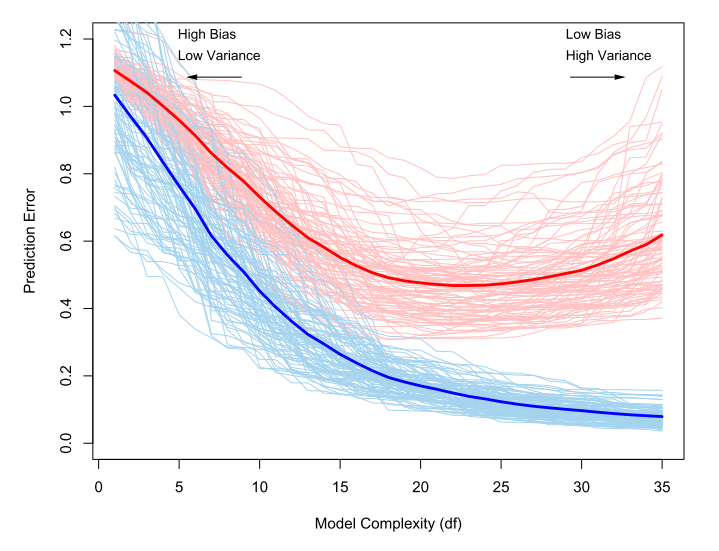
\includegraphics[width=3.2in]{complexity_fit_tradeoff.png}
\end{figure}

\small
Blue is in-sample fit metric and red is oos fit metric. This is Fig 7.1 from Hastie and Tibsharani (2009).

%This provides an honest estimate for one model $\hat{f}$ and one model $\hat{f}$ only.

\end{frame}

\begin{frame}\frametitle{Assessment: OOS Validation}

But knowing where you are on that y-axis would involve knowing the truth. We need to estimate this, so we use oos validation:

\begin{figure}
\centering
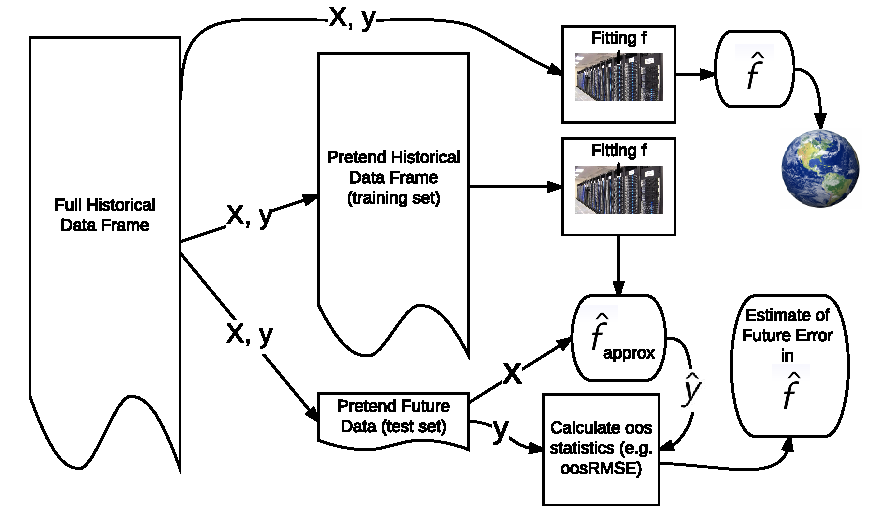
\includegraphics[width=4.1in]{oos_validation}
\end{figure}

%This provides an honest estimate for one model $\hat{f}$ and one model $\hat{f}$ only.

\end{frame}



\begin{frame}\frametitle{Assumptions and Tradeoffs when Splitting}
\footnotesize
We have a choice to split our dataframe into two pieces. Assuming each data point is independent (the running assumption), you should do this completely randomly. When would this assumption not be true? \pause For example, a time series.\\~\\
\vspace{-0.2cm}

Additionally, we need to assume a non-stationary model relationship. So, 

\beqn
Y = f(x_1, \ldots, x_p) + \errorrv \quad \text{and not} \quad Y = f_t(x_1, \ldots, x_p) + \errorrv 
\eeqn

where $f$ changes with time. In essence non-stationarity is a lack of generalization and when predicting, it is a form of extrapolation. \\~\\

How large should the test set be? Usual sizes are 10-30\%. What's the tradeoff? If the test set is larger, then ...
 
\begin{enumerate}\footnotesize
\item the more accurate the assessment of generalization error would be (less variance) and
\item the less accurate the model will be since it's fitting with less data (more bias)
\end{enumerate}

\vspace{-0.1cm}
If the test set is smaller then, vice versa. Note: the in-sample and oos statistics are statistics! Thus, they are random!

\end{frame}


\section{Cross-Validation (CV)}

\begin{frame}\frametitle{Less Randomness in the OOS Statistics}
\small
If we change the observations in the training/test splits, we will get different models and different estimates of future error. \pause Thus, our oosRMSE was really oosRMSE conditional on the idiosyncratic split we happened to get!\\~\\ \pause 

We can at the very least... \pause  get rid of this idiosyncratic error by ... \pause averaging over all training-test splits. If we have $n=100$ and the test set is 10\%, that means we only have $\binom{100}{10} = 1.73 \times 10^{13}$ split configurations to average over! \\~\\ \pause 

\normalsize
We can approximate the averaging over all splits by just taking $\frac{100\%}{10\%} = 10$ random but unique splits called \emph{folds}. \pause Thus, each observation is represented in the test set once (leading to a more stable estimate). \pause This is known as \emph{$K$-fold cross validation (CV)} where here $K = \pause \frac{100\%}{10\%} = 10$ (and this procedure seems to be the industry standard).
	
\end{frame}


\begin{frame}\frametitle{10-fold CV}

\begin{figure}
\centering
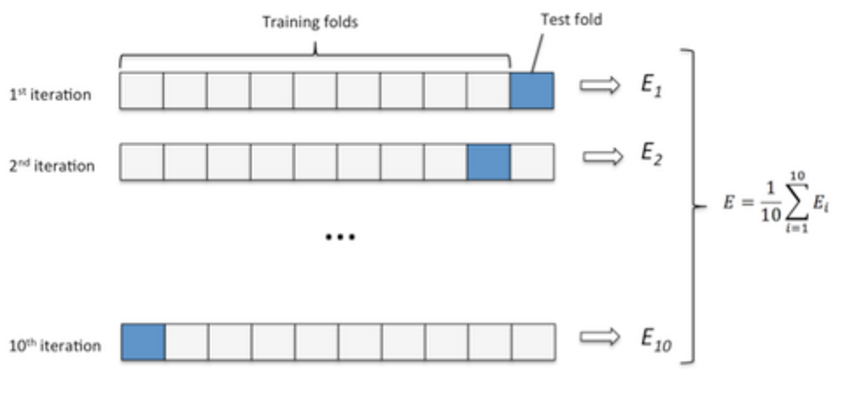
\includegraphics[width=2.9in]{10_fold_cv2.png}
\end{figure}

\vspace{-0.3cm}
\small
$K=10$ is arbitrary (but remember where it was based on: the 10-30\% test set recommendation). In practice, I've only used 5 or 10 fold CV. \\~\\ \pause

\vspace{-0.3cm}
This does not really solve any of our big problems but gives us a little boost in terms of a reduction in standard error of our generalization error estimate. \pause That's OK; we can take all the help we can get if it's costless!! \\~\\

\vspace{-0.4cm}\footnotesize
Note 1: If $K=n$ then we the test set as one sample; this is known as \qu{leave on out CV} (LOOCV) and it not recommended --- high variance and \pause computat- ional cost! \pause Note 2: bleeding edge of stats --- find CI's for generalization error. \pause Note 4: this is not the only way to reduce the variance in oos statistics but it's the one we will use in this class.

	
\end{frame}


\begin{frame}\frametitle{$K=3$-fold CV on a Linear Model Ex. 1/5}

Imagine the following data $n=9$ where we are fitting a response by one feature (ignore the colors):

\begin{figure}
\centering
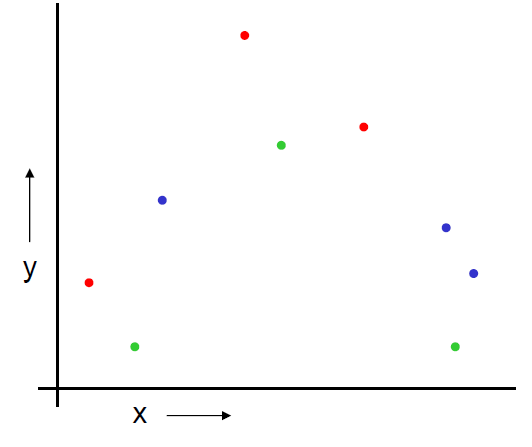
\includegraphics[width=2.1in]{data.PNG}
\end{figure}

Imagine we choose a linear model. 
	
\end{frame}


\begin{frame}\frametitle{$K=3$-fold CV on a Linear Model Ex. 2/5}

In the first fold, the red is left out and thus we fit a line to the blue and green points:

\begin{figure}
\centering
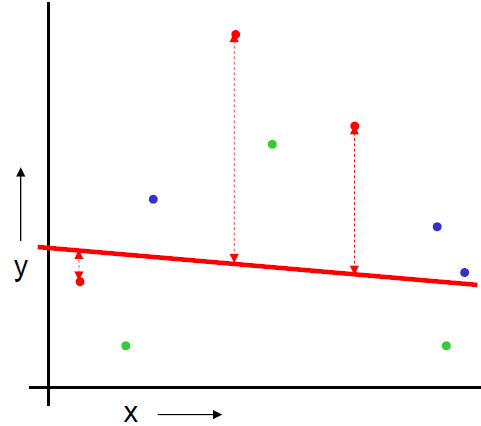
\includegraphics[width=1.8in]{l1.PNG}
\end{figure}

Then we calculate the residuals to the red points (the test set in this fold) and calculate

\beqn
SSE = (2 - 2.2)^2 + (3.8 - 2.1)^2 + (3.5 - 2.05)^2 = 5.03
\eeqn

\end{frame}


\begin{frame}\frametitle{$K=3$-fold CV on a Linear Model Ex. 3/5}

In the second fold, the green is left out and thus we fit a line to the blue and red points:

\begin{figure}
\centering
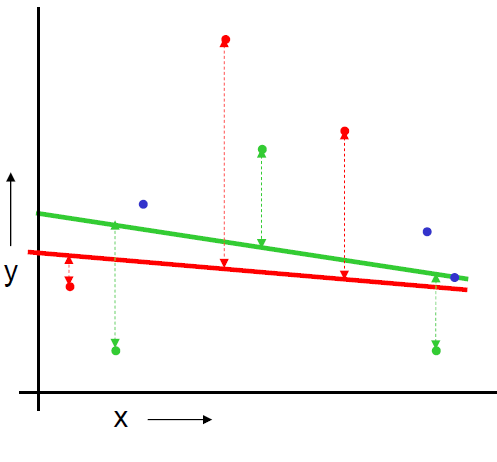
\includegraphics[width=1.8in]{l2.PNG}
\end{figure}

Then we calculate the residuals to the red points (the test set in this fold) and calculate

\beqn
SSE = (1.2 - 2.3)^2 + (3.4 - 2.25)^2 + (1.3 - 2.2)^2 = 3.34
\eeqn
	
\end{frame}


\begin{frame}\frametitle{$K=3$-fold CV on a Linear Model Ex. 4/5}

In the third (last) fold, the blue is left out and thus we fit a line to the green and red points:

\begin{figure}
\centering
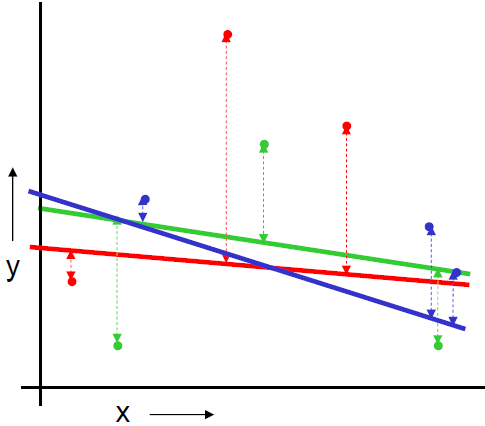
\includegraphics[width=1.8in]{l3.PNG}
\end{figure}

Then we calculate the residuals to the red points (the test set in this fold) and calculate

\beqn
SSE = (2.35 - 2.3)^2 + (2.4 - 1.5)^2 + (2.2 - 1.4)^2 = 1.45
\eeqn
	
\end{frame}


\begin{frame}\frametitle{$K=3$-fold CV on a Linear Model Ex. 1/5}

Then we aggregate all oos results together (SSE's are additive) and we can compute a final oos statistics e.g. the oosRMSE:

\beqn
oosRMSE = \sqrt{\frac{5.03 + 3.34 + 1.45}{9}} = 1.045
\eeqn
	
\end{frame}

\begin{frame}\frametitle{Limits of JMP / Intro to R's MLR Package}

And... \pause JMP can't do $K$-fold CV! (Except in one limited case which doesn't help us right now). But of course R can do it... [R Demo with MLR]
	
\end{frame}


\begin{frame}\frametitle{Validating Multiple Models}
\footnotesize
Let's look at a few models for the White Wine data with no validation (but no cross-validation). Here the response is wine quality as measured by professional raters and features are 11 features (e.g. acidity, sugar, pH and alcohol content).

\vspace{-0.1cm}
\begin{enumerate}\footnotesize
\item[A] plain linear model \pause
\item[B] 6-degree polynomials for all features \pause
\item[C] 6$^{\text{o}}$ polynomials and all 1st order interactions  \pause
\item[D] 6$^{\text{o}}$ polynomials and all interactions up to 3rd degree (AKA 2nd order) \pause
\item[E] 6$^{\text{o}}$ polynomials and all interactions up to 4th degree (AKA 3rd order) \pause
\item[F] 6$^{\text{o}}$ polynomials and all interactions up to 11th order \pause
\end{enumerate}
\footnotesize
\vspace{-0.1cm}
[JMP col validation... fit all models with validation ... save prediction formula cols... analyze model... model comparison... \pause complexity tradeoff illustration] \pause Conclusions? \pause Model C looks the best. \pause Note: another popular assessment metric besides oosRMSE is oosAAE which is just average absoute value difference. Strange ... given that linear models optimize for squared error. \pause 
Show Demo with MLR w/ 10-fold CV \pause \inred{What \textit{precisely} did I do that wasn't legal?} 
	
\end{frame}

\begin{frame}\frametitle{A Possible Spin on Validation}
\small

Recall the proposal from last class:
	
\begin{enumerate}\footnotesize
\item Split dataframe into training and test.
\item Build model A on training.
\item Predict using the test set. 
\item Calculate estimate of future generalization error of model 1.
\item Build a different model B on training.
\item Predict using the test set. 
\item Calculate estimate of future generalization error of model 2.
\item ... steps 5-7 for model 3
\item ... steps 5-7 for model 4
\item ...
\item ... steps 5-7 for model M
\item Pick whichever model has better generalization error.
\end{enumerate}

This is a form of \emph{Model Selection}. What was wrong with it?

\end{frame}

\begin{frame}\frametitle{Looking into the Future is Not Legal}

The oos validation is only valid if...

\begin{figure}
\centering
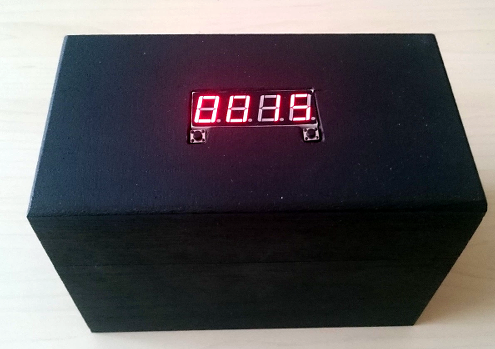
\includegraphics[width=1.2in]{lockbox.png}
\end{figure}

you treat the test set as a lockbox. Once you open it up, that's it! And we opened it up $M$ times!\\~\\ \pause

This is indeed a \emph{Model Selection} procedure but ... \pause our estimate of future generalization error is invalid. How can we do both?
	
\end{frame}

\section{Three Splits and CV}

\begin{frame}\frametitle{In One Fold Let's Focus on the Training Set}
\vspace{-0.2cm}
\begin{figure}
\centering
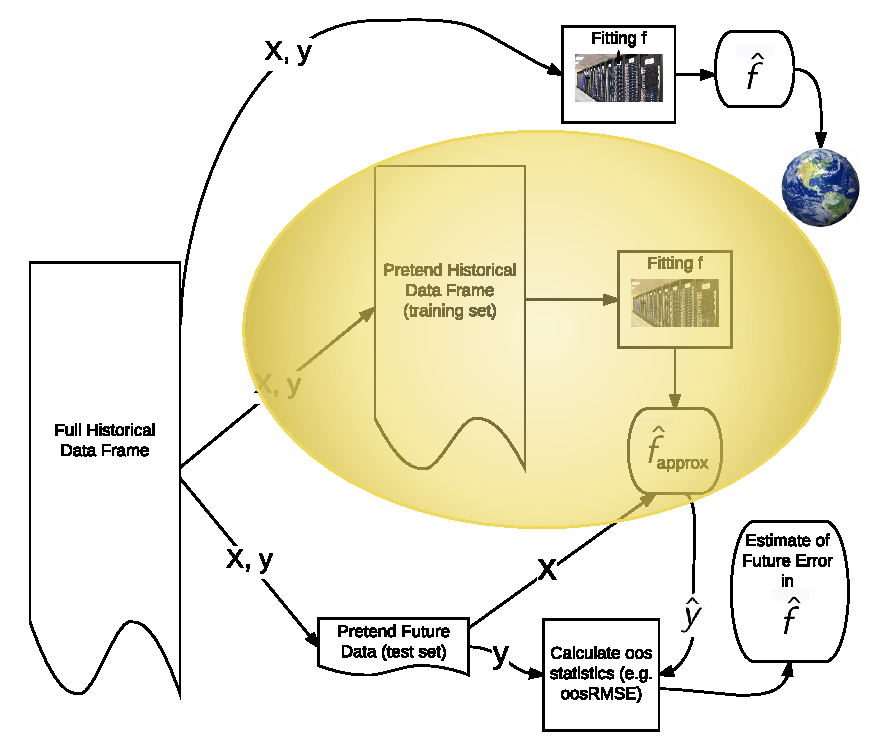
\includegraphics[width=3.1in]{oos_validation_highlighted}
\end{figure}

\small
\vspace{-0.3cm}
\pause This procedure was completely valid as long as we did not touch the test set, right? \pause As long as we operate only within the training set... we're OK!
	
\end{frame}

\begin{frame}\frametitle{Training $\Rightarrow$ Training \& Validation}
\vspace{-0.5cm}
\begin{figure}
\centering
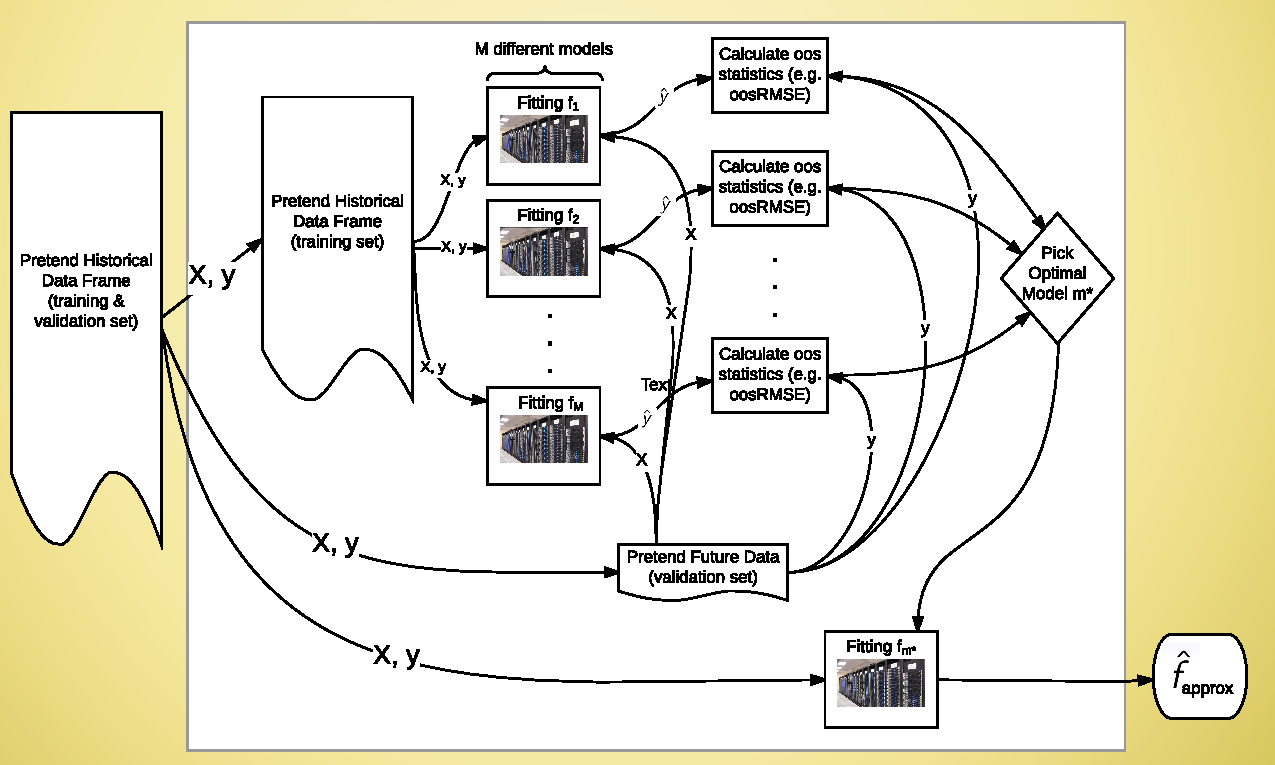
\includegraphics[width=4.4in]{training_validation}
\end{figure}
	
\end{frame}

\begin{frame}\frametitle{3-way Splitting: The Full Picture}
\vspace{-0.8cm}
\begin{figure}
\centering
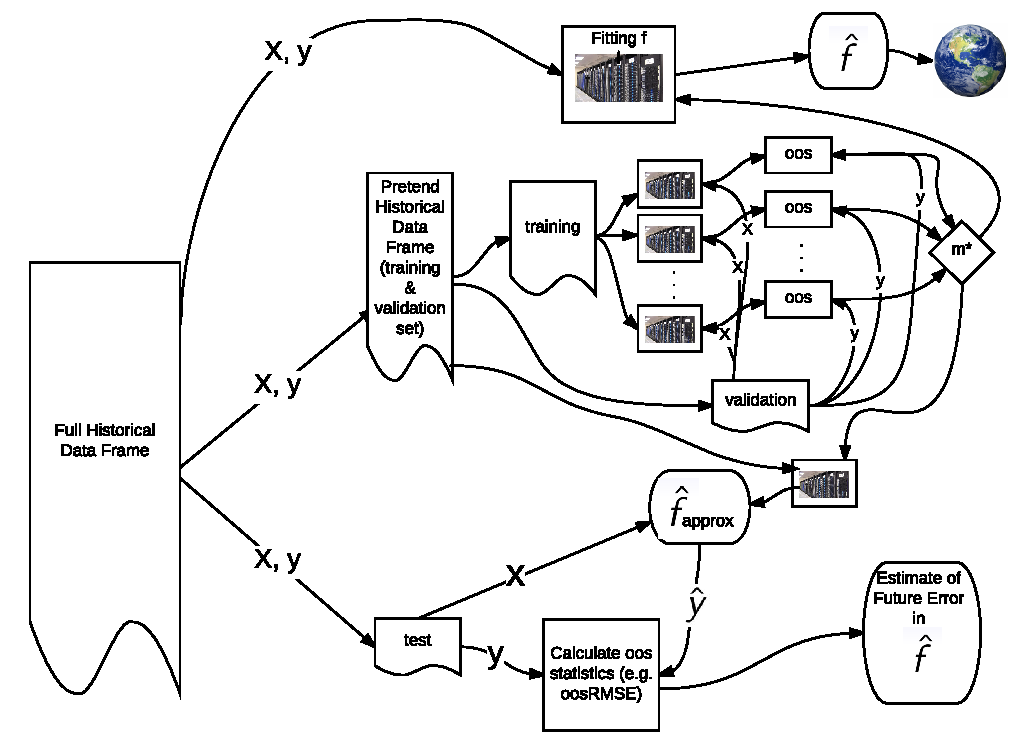
\includegraphics[width=4.26in]{3_way_validation}
\end{figure}
	
\end{frame}

\begin{frame}\frametitle{Why Training-Validation-Test Splitting?}

\begin{itemize}
\item Training set: \pause provides fits for many models where overfitting is \qu{okay}
\item Validation set: \pause provides out-of-sample validation for each of the models. If the models are overfit, they will get wrecked at this stage.
\item Test set: \pause this lockbox provides a layer of security against overfitting within the training-validation union set. \pause
\end{itemize}

Just like in the previous 2-way training-test split, you can overfit the training, get killed on the test set and be stuck. How could you similaryl overfit here? \pause Be careful of optimizing to the validation set. Models $1, 2, \ldots, M$ should still be reasonable thought-through models.


\end{frame}


\begin{frame}\frametitle{Sizes of Training-Validation-Test Splits}

Previously, we had the test set being 10-30\%. This recommendation remains. Thus, the training-validation sets together should make up 70-90\% of which a portion is the validation set \pause (which is like a test set) and should be \pause 10-30\% of the total. \pause Thus we arrive at proportions like 50-25-25 or 50-30-20 or 70-20-10. \pause There is no exact guidance here. \\~\\ \pause

The same tradeoffs apply to the test set size but now we have new tradeoffs for the training set size vs. the validation set size:

\begin{itemize}
\item The larger the training set, \pause the better the fit of the model (less bias) but the more variance in its assessment versus its peers
\item The smaller the training set, \pause the worse the fit of the model (more bias) but the less variance in its assessment versus its peers
\end{itemize}
	
\end{frame}

\begin{frame}\frametitle{Back to Wine...}

We can do a single 3-partition split in JMP using the validation column... then data filter... then fit the 6 models again... then use model comparison to select best model ... then undo the filter ... then use model comparison again to find our test set error (the guess of the generalization error)... then build the full model for public consumption.
	
\end{frame}

\begin{frame}\frametitle{Can you CV this 3-Split Procedure?}

\pause

\begin{minipage}{0.6\textwidth}
\begin{figure}
\centering
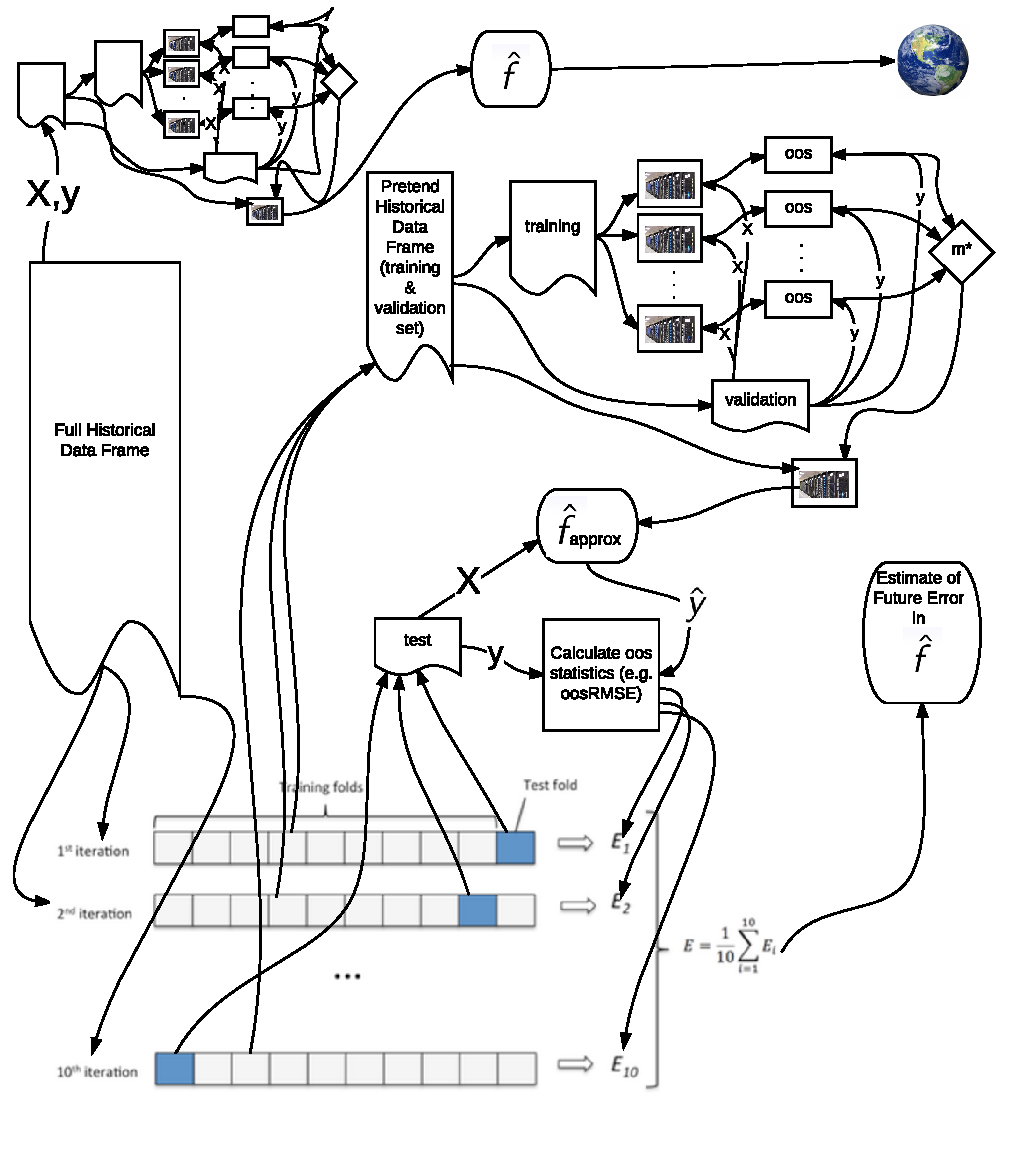
\includegraphics[width=2.56in]{nested_resampling}
\end{figure}
\end{minipage}~
\begin{minipage}{0.35\textwidth}
\small
Yes. It is called \qu{nested resampling} and $K=10$ fold CV is illustrated here. But... \pause what are you now evaluating? \\~\\

\pause Without CV, it was just model $m^*$. But here $m^*$ varies with the 10 folds! \pause You are testing the entire procedure i.e. given models $1, 2, \ldots, M$, pick the best one and ship it. How well you do in the future is estimated by the CV test set.
\end{minipage}


	
\end{frame}



\begin{frame}\frametitle{Not the First Means for Model Selection}

CV with nested resampling is not generally done in the way it was described here as a means to evaluate a model selection procedure. \pause Beyond scope of course: it is usually done to compare tuning settings in a non-parametric machine learning algorithm. We will see what this means next class. \\~\\ \pause

Neither R nor JMP (to my knowledge) can do this out-of-the-box. In R, even with MLR, you have to program it (MLR uses it for tuning an algorithm). Maybe I will write to them?
	
\end{frame}

\begin{frame}\frametitle{Nested Resampling for Tuning}

\begin{figure}
\centering
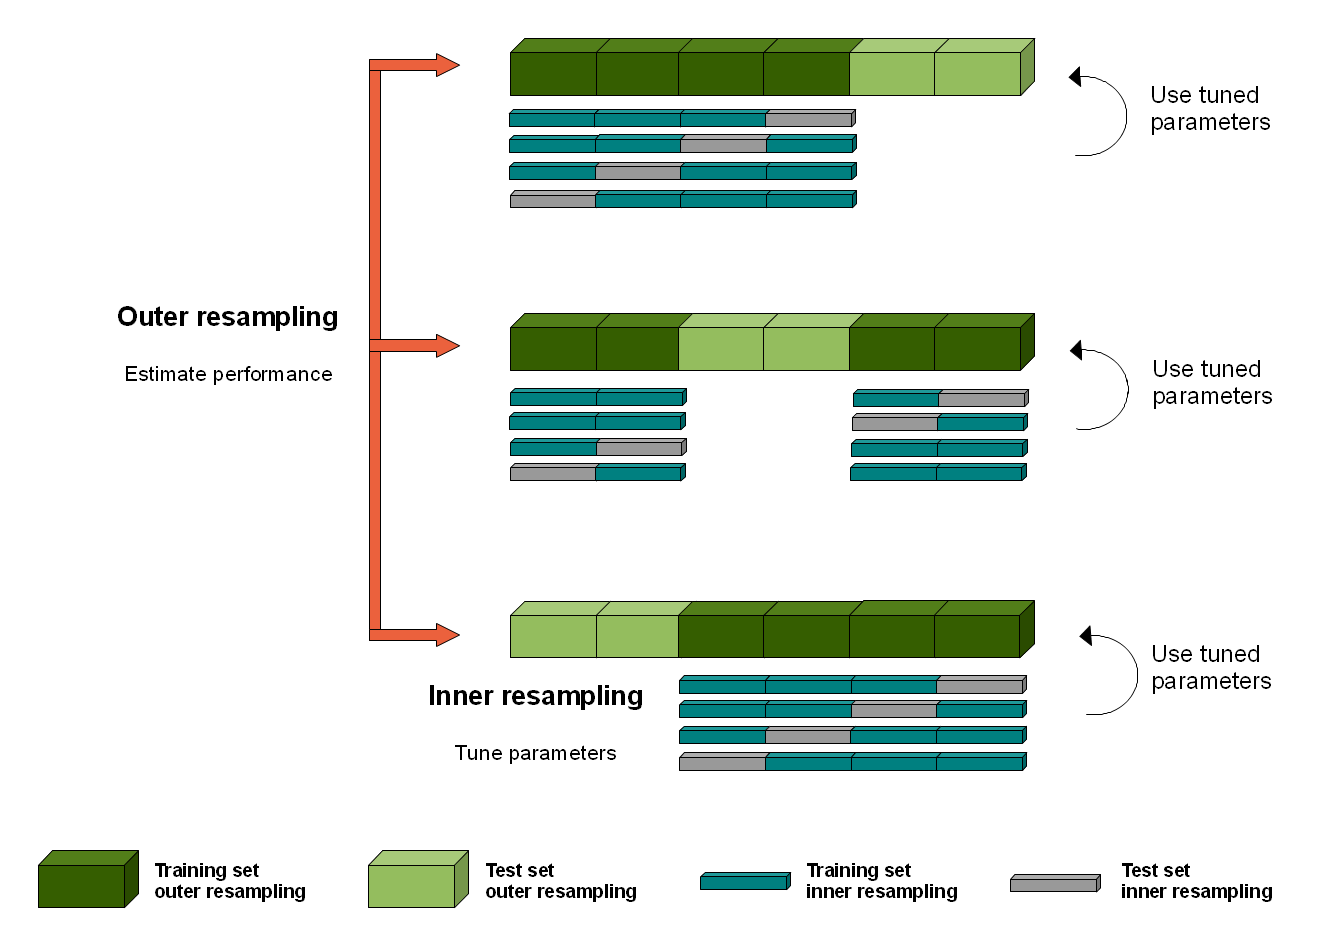
\includegraphics[width=3.56in]{nested_resampling_for_tuning.png}
\end{figure}

(from \href{https://mlr-org.github.io/mlr-tutorial/devel/html/nested_resampling/index.html}{MLR's tutorial website}).
\end{frame}

\section{Automatic Model Selection}

\begin{frame}\frametitle{3-way splits for model selection \& evaluation}
\small
Forget CV for a moment since it complicates things ... the \qu{inner split} consisted of the training-validation. We used this to \qu{select} a model based on lowest oos error (RMSE, or highest $R^2$). 

\vspace{-0.2cm}
\begin{figure}
\centering
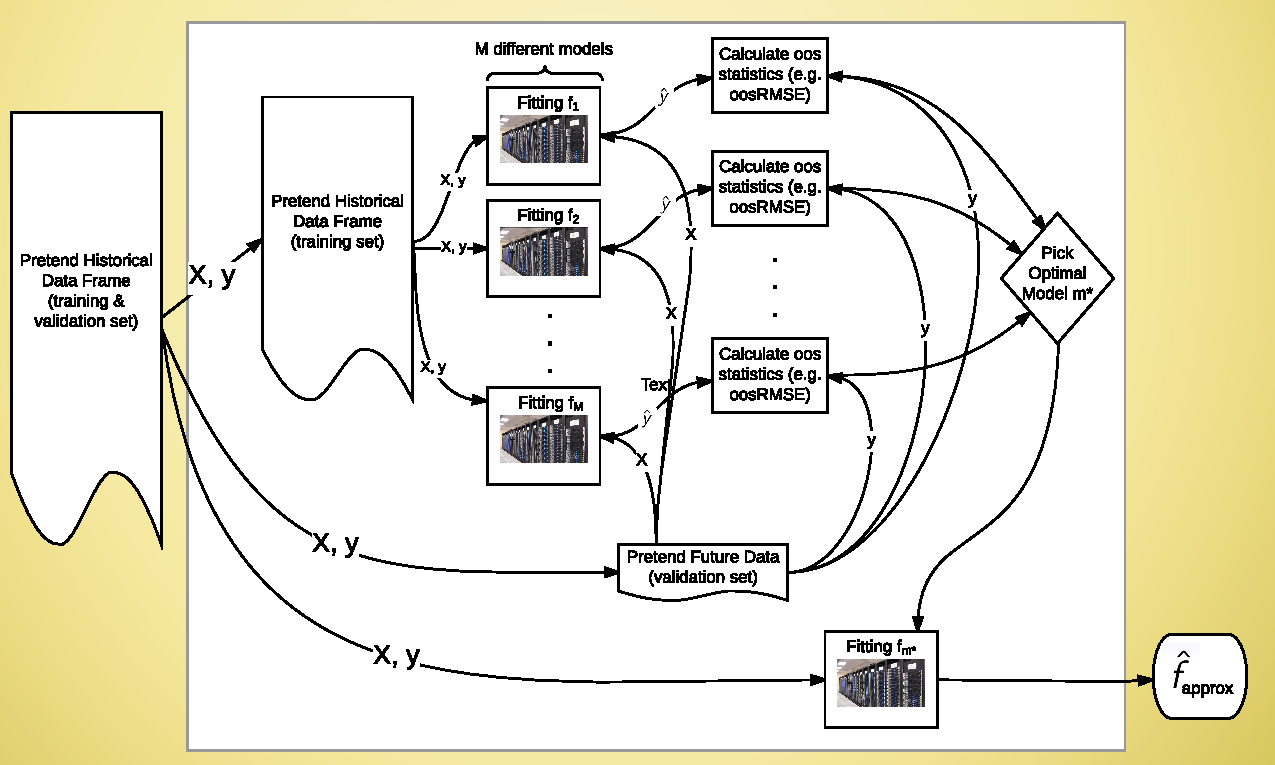
\includegraphics[width=2.1in]{training_validation}
\end{figure}
\vspace{-0.2cm}
What's the cost? \pause We had to use only 70-90\% of the data (save the test set) to build the model. But what's the bigger cost?? \pause You had to provide models $1, 2, \ldots, M$!! This is no trivial task. So far I've been making them up! I've been using elebaorate linear models which pivoted from param- etric to non-parametric with the addition of curves and interactions. Forget finding the best model... how do we know we even employed good candidates?? \pause \inred{We don't!}

\end{frame}


\begin{frame}\frametitle{Modeling Framework Refresher}
\small
Recall the general regression model:

\beqn
Y = f(x_1, \ldots, x_p) + \errorrv
\eeqn

A couple lectures ago, we made the parametric assumption that: \pause

\beqn
Y = s(x_1, \ldots, x_p; \theta_1, \ldots, \theta_\ell) + \tilde{\errorrv}
\eeqn

where the $\tilde{\errorrv}$ term now includes the previous $\errorrv$ plus $f-s$, the misspecification error. \pause The parametric model $s$ we employed was the linear model and the $\theta$'s we called $\beta$'s: \pause

\beqn
Y = \beta_0 + \beta_1 x_1 + \ldots + \beta_p x_p + \tilde{\errorrv}
\eeqn

Last lecture, we started adding interactions and polynomials (as well as other transformations e.g. log which we did not cover). \pause This was a means of \qu{expanding} the feature set \qu{visible} to the model using \qu{derived} features: \pause

\beqn
\braces{x_1, \ldots, x_p} \Rightarrow \braces{x'_1, \ldots, x'_{p'}} ~~ \text{where $p' > p$ and maybe much, much greater}
\eeqn

\end{frame}

\begin{frame}\frametitle{\qu{Non-parametric} Linear Regression}

Once we expand this feature set, we can now fit a larger linear model:

\beqn
Y = \beta_0 + \beta_1 x'_1 + \ldots\ldots\ldots\ldots\ldots\ldots\ldots + \beta_p x'_{p'} + \tilde{\errorrv}
\eeqn

Given more degrees of freedom with this expanded feature set allows the linear model to fit more complicated real-world functions. \pause This is essentially a means of doing non-parametric parametric modeling (it's oxymoronic). It's technically parametric but conceptually it's non-parametric since we don't have our parametric benefits: parsimony, inference nor interpretation. Hopefully $\tilde{\errorrv}$ will be close to $\errorrv$, the irreducible noise. \\~\\ \pause

Back to our problem... we can curb overfitting by ... \pause using 3-way split oos validation but we need to select good models... how to do so? \pause One approach is termed \emph{subset selection methods}.
\end{frame}


\begin{frame}\frametitle{Stepwise Regression}

First we expand the feature set from $\braces{x_1, \ldots, x_p} \Rightarrow \braces{x'_1, \ldots, x'_{p'}}$. \pause Then we attempt to find the \qu{best} model consisting of a subset of these features. However there are $2^{p'}$ possible models. For $p'=20$ that's about 1,000,000. \pause So we try to find a model \textit{close} to the optimal using a \qu{heuristic} (a rule of thumb that seems to generally be useful).\\~\\ \pause

That heuristic is called \emph{stepwise} model construction. \pause We begin with \emph{forward stepwise} model construction: \pause

\begin{enumerate}
\item Find the \qu{best} feature from the list of expanded features.\pause
\item Find the \qu{next best} feature from the remaining expanded features.\pause
\item Repeat step 2 until you believe you are overfitting.\pause
\end{enumerate}




\end{frame}

\begin{frame}\frametitle{Estimating Overfitting (again)}
\small
If you choose the feature to give you the best in-sample $R^2$, you will eventually take all the features (until $n = p+1$) and you will get $R^2 = 100\%$. We need a metric to tell us when we may be overfitting and halt at that moment. \pause Here are a few:

\begin{enumerate}
\item oos RMSE (keep a holdout set and quit when this starts increasing) \pause
\item Only include a variable if its $t$ stat (or partial $F$ stat) is significant \pause
\item Use $AICc$.
\end{enumerate}

\beqn
-AIC = 2\loglik{\betahat; \y, \x} - 2p
\eeqn

The first component (the log-likelihood) represents in-sample fit. \pause $\loglik{}$ is like $R^2$ though... as the fit gets closer to the points, the likelihood goes to 1 (and the log likelihood goes to 0). \pause The $2p$ term is a reality check. If you have more features, you are going to overfit. So each additional feature must be justified in terms of the increase in log-likelihood. \pause Thus, good models maximize $-AIC$ (i.e. minimize $AIC$).\\~\\


	

\end{frame}

\begin{frame}\frametitle{$AICc$ for linear models}
\small
For linear regression under OLS, we can calculate the log-likelihood explicitly (we approximately did this in Lecture 2) to obtain:

\beqn
AIC = n\natlog{RMSE^2} + 2p
\eeqn

\pause So once again, we want this to be small. If we decrease $RMSE$ by adding a feature, it needs to counteract an increase of 2 by $p \rightarrow p+1$. If it can't, we're probably overfitting. \pause $AIC$ works well with large sample sizes. For small sample sizes, we use a corrected version $AICc$ defined as:

\beqn
AICc = AIC + \frac{2p(p+1)}{n-p-1}
\eeqn

Needless to say, this is all approximate since we are assuming OLS and a whole bunch of other things (beyond scope of course). \pause Note: there are also BIC and Mallow's $C_p$ which are similar metrics, but we will not cover them. \pause \[JMP demo for white wine dataset. Make sure \qu{no rules} checked.\]
	
\end{frame}

\begin{frame}\frametitle{}

	
\end{frame}


\end{document} %%%%%%%%%%%%%%%%%%%%%%%%%%%%%%%%%






\begin{frame}\frametitle{}

	
\end{frame}


\begin{frame}\frametitle{}

	
\end{frame}

\begin{frame}\frametitle{}

	
\end{frame}


\begin{frame}\frametitle{}

	
\end{frame}

\begin{frame}\frametitle{}

	
\end{frame}


\begin{frame}\frametitle{}

	
\end{frame}

\begin{frame}\frametitle{}

	
\end{frame}


\begin{frame}\frametitle{}

	
\end{frame}

\begin{frame}\frametitle{}

	
\end{frame}


\begin{frame}\frametitle{}

	
\end{frame}

\begin{frame}\frametitle{}

	
\end{frame}


\begin{frame}\frametitle{}

	
\end{frame}

\begin{frame}\frametitle{}

	
\end{frame}


\begin{frame}\frametitle{}

	
\end{frame}

\begin{frame}\frametitle{}

	
\end{frame}